\section{Casi d'uso}
\subsection{Scopo}

La presente sezione ha come obiettivo l'identificazione e la descrizione di tutti i casi d'uso individuati dall'analisi del gruppo sul capitolato proposto.
    
\subsection{Attori}
Come concordato con il proponente, la web app$^{G}$ deve essere utilizzata sia da utenti clienti che da utenti ristoratori, sono stati quindi identificati per il Sistema i seguenti attori:
\begin{itemize}
    \item \textbf{Utente non riconosciuto:} è un utente che non ha effettuato l'accesso al Sistema. Può essere sia un utente non registrato sia un utente registrato che non ha ancora effettuato l'accesso.\\
    Può ricercare specifici ristoranti e visualizzarli;
    \item \textbf{Utente autenticato:} è un utente che ha effettuato l'accesso al Sistema ma non ha ancora selezionato un profilo.\\ 
    Può creare, modificare o eliminare profili cliente o ristoratore;
    \item \textbf{Cliente:} è un utente che ha effettuato l'accesso al Sistema ed ha selezionato un profilo cliente.\\
    Può effettuare le operazioni di prenotazione ed ordinazione e le loro attività correlate;
    \item \textbf{Ristoratore:} è un utente che ha effettuato l'accesso al Sistema ed ha selezionato un profilo ristoratore.\\
    Può gestire il proprio ristorante e le prenotazioni ad esso associate.
\end{itemize}
\subsection{Lista dei casi d'uso}


% registazione - login - navigazione del sito
\textbf{UC1-Registrazione account}
\begin{itemize}
    \item \textbf{Attore principale: }Utente non riconosciuto.
    \item \textbf{Precondizioni: }L'utente è connesso al sistema.
    \item \textbf{Postcondizioni: }L'account dell'utente e le informazioni ad esso collegate, sono registrati nel sistema.
    \item \textbf{Scenario principale:} 
        \begin{enumerate}
            \item L'utente sceglie l'opzione di registrazione di un account;
            \item Il sistema chiede all'utente di inserire una email ed una password;
            \item L'utente inserisce l'email e la password;
            \item L'utente conferma i valori inseriti;
            \item Il sistema comunica all'utente che la registrazione è andata 
            a buon fine.
            \item Il cliente visualizza un profilo di tipo cliente creato di default dal sistema.
        \end{enumerate}
    \item \textbf{Estensioni:}
        \begin{itemize}
                \item UCE1.1-Campo mancante;
                \item UC1.2-Email già registrata nel sistema.
        \end{itemize}
\end{itemize}
    
\textbf{UCE1.1-Campo mancante}
\begin{itemize}
    \item \textbf{Descrizione: }Per effettuare la registrazione,deve essere inserito un valore sia per la password che per l'email.
    \item \textbf{Scenario alternativo:}
    \begin{enumerate}
        \item Al momento della conferma,il sistema rileva che uno dei campi (o entrambi) risulta non compilato;
        \item Il sistema comunica la natura dell'errore all'utente;
        \item L'utente visualizza i campi di mail e password con i valori inseriti precedentemente.
    \end{enumerate}
\end{itemize}

\textbf{UC1.2-Email già registrata nel sistema}
\begin{itemize}
    \item \textbf{Descrizione: }L'utente non può registrare un account inserendo una email già usata da un altro utente.
    \item \textbf{Scenario alternativo:}
    \begin{itemize}
        \item L'email inserita dall'utente al momento della registrazione risulta associata ad un
        account già registrato nel sistema;
        \item Il sistema comunica la natura dell'errore all'utente;
        \item L'utente è reindirizzato alla homepage di registrazione.
    \end{itemize}
\end{itemize}
\break

\textbf{UC2-Login}
\begin{itemize}
\item \textbf{Attore principale:} Utente non riconosciuto.
\item \textbf{Precondizioni:} L'utente è connesso al sistema.
\item \textbf{Postcondizioni:} L'utente è autenticato presso il sistema.
\item \textbf{Scenario principale:}
\begin{enumerate}
    \item L'utente sceglie l'opzione di login;
    \item L'utente inserisce la sua password;
    \item l'utente inserisce la sua email;
    \item L'utente conferma i dati inseriti al sistema;
    \item Il sistema verifica l'esistenza di un account con i suddetti dati;
    \item L'utente visualizza la lista dei profili afferenti al suo account.
\end{enumerate}
    \item \textbf{Estensione: }UCE2-Credenziali non corrette.
\end{itemize}

\textbf{UCE2-Credenziali non corrette}
\textbf{Descrizione: }Il login può non andare a buon fine se l'email inserita dall'utente non è registrata 
o la password non è corretta; per questioni di sicurezza, all'utente viene notificato un errore generico.
\textbf{Scenario secondario:}
\begin{enumerate}
    \item Dopo la conferma dei dati inseriti dall'utente,il sistema verifica 
    che l' email non è presente nel sistema o che la password associata non è corretta;
    \item Il sistema comunica all'utente che le credenziali inserite non sono corrette;
    \item L'utente può riprovare ad effettuare il login ,inserendo di nuovo l'email e la password.
\end{enumerate}

\textbf{UC16-Visualizzazione lista ristoranti}
\begin{itemize}
\item \textbf{Attore principale:} Utente non riconosciuto / cliente.
\item \textbf{Precondizioni:} L'utente è connesso al sistema.
\item \textbf{Postcondizioni:} L'utente visualizza una lista di ristoranti.
\item \textbf{Scenario principale:}
\begin{enumerate}
    \item L'utente seleziona la funzionalità di visualizzazione di una lista di ristoranti;
    \item L'utente visualizza una lista di ristoranti,ordinati secondo la loro valutazione media in ordine decrescente.
\end{enumerate}
\end{itemize}

\textbf{UC17-Ricerca ristorante}
\begin{itemize}
\item \textbf{Attore principale:}U non riconosciuto / cliente.
\item \textbf{Precondizioni:} L'utente è connesso al sistema.
\item \textbf{Postcondizioni:} L'utente visualizza la lista dei ristoranti corrispondenti ai criteri inseriti
dell'utente.
\item \textbf{Scenario principale:}
\begin{enumerate}
    \item L'utente seleziona la funzionalità di ricerca di un ristorante;
    \item L'utente può effettuare la ricerca inserendo uno o più parametri ,corrispondenti
    ai seguenti criteri:
    \begin{itemize}
        \item Il nome del ristorante (vedi UC17.1-Ricerca per nome);
        \item La città del ristorante (vedi UC17.2-Ricerca per città);
        \item La valutazione media del ristorante (vedi UC17.3-Ricerca per valutazione);
        \item La tipologia di cucina (vedi UC17.4-Ricerca per tipologia di cucina);
        \item L' orario (vedi UC17.5-Ricerca ristorante per orario) ;
        \item La data (vedi UC17.6-Ricerca ristorante per data); 
    \end{itemize}
    \item  Il sistema filtra la lista di ristoranti secondo i criteri inseriti;
    \item L'utente visualizza la lista dei ristoranti che rispettano i criteri da lui inseriti.
\end{enumerate}
\end{itemize}

\textbf{UC17.1-Ricerca ristorante per nome}
\begin{itemize}
\item \textbf{Attore principale:}uìUtente non riconosciuto / cliente.
\item \textbf{Precondizioni:} L'utente è connesso al sistema.
\item \textbf{Postcondizioni:} L'utente visualizza la lista dei ristoranti corrispondenti 
alla ricerca per nome da lui inserito.
\item \textbf{Scenario principale:}
\begin{enumerate}
    \item L'utente seleziona la funzionalità di ricerca di un ristorante;
    \item L'utente inserisce il testo che deve essere contenuto nel nome; 
    \item  Il sistema filtra la lista di ristoranti secondo il criterio inserito;
    \item L'utente visualizza la lista dei ristoranti corrispondenti al nome da lui inserito.
\end{enumerate}
\end{itemize}

\textbf{UC17.2-Ricerca ristorante per città}
\begin{itemize}
\item \textbf{Attore principale:}Utente non riconosciuto / cliente.
\item \textbf{Precondizioni:} L'utente è connesso al sistema.
\item \textbf{Postcondizioni:} L'utente visualizza la lista dei ristoranti corrispondenti alla città da lui inserita.
\item \textbf{Scenario principale:}
\begin{enumerate}
    \item L'utente seleziona la funzionalità di ricerca di un ristorante;
    \item L'utente inserisce la città come parametro di ricerca;
    \item Il sistema filtra la lista di ristoranti secondo il criterio inserito;
    \item L'utente visualizza la lista dei ristoranti corrispondenti alla città inserita.
\end{enumerate}
\end{itemize}

\textbf{UC17.3-Ricerca ristorante per valutazione}
\begin{itemize}
\item \textbf{Attore principale:}Utente non riconosciuto / cliente.
\item \textbf{Precondizioni:} L'utente è connesso al sistema.
\item \textbf{Postcondizioni:} L'utente visualizza la lista dei ristoranti la cui valutazione è maggiore o uguale alla
valutazione da lui inserita.
\item \textbf{Scenario principale:}
\begin{enumerate}
    \item L'utente seleziona la funzionalità di ricerca di un ristorante;
    \item L'utente inserisce il valore della valutazione che desidera;
    \item Il sistema filtra la lista di ristoranti secondo il criterio inserito;
    \item  L'utente visualizza la lista dei ristoranti con valutazione maggiore o uguale a quella da lui inserita.
\end{enumerate}
\end{itemize}

\textbf{UC17.4-Ricerca ristorante per tipologia di cucina}
\begin{itemize}
\item \textbf{Attore principale:}Utente non riconosciuto / cliente.
\item \textbf{Precondizioni:} L'utente è connesso al sistema.
\item \textbf{Postcondizioni:} L'utente visualizza la lista dei ristoranti che offrono la tipologia di cucina
da lui inserita.
\item \textbf{Scenario principale:}
\begin{enumerate}
    \item L'utente seleziona la funzionalità di ricerca di un ristorante;
    \item L'utente seleziona una o più tipologie di cucina alle quali è interessato;
    \item Il sistema filtra la lista di ristoranti secondo il criterio inserito; 
    \item L'utente visualizza la lista dei ristoranti che offrono la/e tipologia/e di cucina da egli cercata.
\end{enumerate}
\end{itemize}

\textbf{UC17.5-Ricerca ristorante per orario}
\begin{itemize}
\item \textbf{Attore principale: }Utente non riconosciuto / cliente.
\item \textbf{Precondizioni:} L'utente è connesso al sistema.
\item \textbf{Postcondizioni:} L'utente visualizza la lista dei ristoranti che hanno posti disponibili nell'orario 
da lui scelto.
\item \textbf{Scenario principale:}
\begin{enumerate}
    \item L'utente seleziona la funzionalità di ricerca di un ristorante;
    \item L'utente seleziona l'orario ;
    \item Il sistema filtra la lista di ristoranti secondo il criterio inserito;
    \item L'utente visualizza la lista dei ristoranti che hanno posti disponibili nell'orario da lui
    selezionato.
\end{enumerate}
\end{itemize}

\textbf{UC17.6-Ricerca ristorante per data}
\begin{itemize}
\item \textbf{Attore principale:} Utente non riconosciuto / cliente.
\item \textbf{Precondizioni:} L'utente è connesso al sistema.
\item \textbf{Postcondizioni:} L'utente visualizza la lista dei ristoranti che hanno posti disponibili
nella data da lui selezionata.
\item \textbf{Scenario principale:}
\begin{enumerate}
    \item L'utente seleziona la funzionalità di ricerca di un ristorante;
    \item L'utente seleziona la data;
    \item Il sistema filtra la lista di ristoranti secondo il criterio inserito;
    \item L'utente visualizza la lista dei ristoranti che hanno posti disponibili
    nella data selezionata .
\end{enumerate}
\end{itemize}

\textbf{U18-Visualizzazione ristorante}
\begin{itemize}
\item \textbf{Attore principale:} Utente non riconosciuto / cliente.
\item \textbf{Precondizioni:} L'utente è connesso al sistema e sta visualizzando una lista di ristoranti.
\item \textbf{Postcondizioni:} L'utente visualizza le informazioni relative al ristorante selezionato.
\item \textbf{Scenario principale:}
\begin{enumerate}
    \item L'utente seleziona un ristorante dalla lista che sta visualizzando ;
    \item L'utente visualizza le informazioni relative al ristorante :
    \begin{itemize}
        \item Il nome;
        \item il recapito telefonico;
        \item L'indirizzo;
        \item gli orari di servizio;
        \item la/le tipologie di cucine offerte;
        \item la valutazione media.
    \end{itemize}
    \item L'utente può scegliere di visualizzare il menù completo (vedi UC18.1-Visualizzazione menù);
    \item L'utente può scegliere di visualizzare le recensioni rilasciate da altri utenti (vedi UC18.2-Visualizzazione recensioni).
\end{enumerate}
\end{itemize}

\textbf{UC18.1-Visualizzazione menù}
\begin{itemize}
\item \textbf{Attore principale:} Utente non riconosciuto / cliente.
\item \textbf{Precondizioni:} L'utente sta visualizzando le informazioni di un ristorante.
\item \textbf{Postcondizioni:} L'utente visualizza il menù del ristorante.
\item \textbf{Scenario principale:}
\begin{enumerate}
    \item L'utente seleziona la funzionalità di visualizzazione del menù del ristorante;
    \item L'utente visualizza la lista completa delle pietanze presenti nel menù;
    \item L'utente può effettuare la ricerca di una pietanza (vedi UC18.1.1-Ricerca pietanza);
    \item L'utente può visualizzare i dettagli relativi ad una singola pietanza presente
     nel menù (vedi UC18.1.2-Visualizzazione pietanza).
\end{enumerate}
\end{itemize}

\textbf{UC18.1.1-Ricerca pietanza}
\begin{itemize}
\item \textbf{Attore principale:} Utente non riconosciuto / cliente.
\item \textbf{Precondizioni:} L'utente sta visualizzando il menù di un ristorante.
\item \textbf{Postcondizioni:} L'utente visualizza la lista delle pietanze corrispondenti ai parametri di ricerca.
\item \textbf{Scenario principale:}
\begin{enumerate}
    \item L'utente seleziona la funzionalità di ricerca di una pietanza ;
    \item L'utente può effettuare la ricerca per nome;
    \item L'utente può effettuare la ricerca selezionando gli allergeni che non vuole 
    siano presenti nelle pietanze del menù;
    \item Il sistema filtra la lista delle pietanze secondo i parametri inseriti;
    \item L'utente visualizza la lista delle pietanze corrispondenti ai criteri di ricerca
    (la lista eventualmente può essere vuota).
\end{enumerate}
\end{itemize}



\textbf{UC18.1.2-Visualizzazione pietanza}
\begin{itemize}
\item \textbf{Attore principale:} Utente non riconosciuto / cliente.
\item \textbf{Precondizioni:} L'utente sta visualizzando il menù di un ristorante.
\item \textbf{Postcondizioni:} L'utente visualizza le informazioni relative alla pietanza selezionata.
\item \textbf{Scenario principale:}
\begin{enumerate}
    \item L'utente seleziona una pietanza in particolare, presente nel menù che sta visualizzando;
    \item L'utente visualizza le seguenti informazioni ad essa relativa:
    \begin{itemize}
        \item La lista degli ingredienti in essa presenti;
        \item La lista degli allergeni;
        \item Il prezzo.
    \end{itemize}
\end{enumerate}
\end{itemize}

\textbf{UC18.2-Visualizzazione recensioni}
\begin{itemize}
\item \textbf{Attore principale:} Utente non riconosciuto / cliente.
\item \textbf{Precondizioni:} L'utente sta visualizzando le informazioni relative ad un ristorante.
\item \textbf{Postcondizioni:} L'utente visualizza le ultime 5 recensioni fatte in ordine temporale decrescente da altri utenti.
\item \textbf{Scenario principale:}
\begin{enumerate}
    \item L'utente seleziona la funzionalità di visualizzazione delle recensioni fatte da altri utenti
    sulla loro esperienza presso il ristorante;
    \item Di default,se presenti più di 5 recensioni, il sistema ne presenta una lista con le ultime 5 fatte in ordine temporale decrescente;
    \item L'utente visualizza le suddette recensioni ,corredate dalle seguenti informazioni:
    \begin{itemize}
        \item Un voto da 1 a 5 sul menù;
        \item Un voto da 1 a 5 sul servizio;
        \item Un voto da 1 a 5 sul prezzo;
        \item Un eventuale commento testuale.
    \end{itemize}
\end{enumerate}
\end{itemize}

% profili

\textbf{UC3-Modifica account }
\begin{itemize}
    \item \textbf{Attore principale:} utente autenticato.
    \item \textbf{Precondizioni:} l'utente è autenticato all'interno del sistema.
    \item \textbf{Postcondizioni:} le modifiche fatte alle informazioni dell'account dell'utente sono
    salvate dal sistema.
    \item \textbf{Scenario principale:}
        \begin{enumerate}
            \item L'utente seleziona l'opzione di modifica dei dati del suo account;
            \item L'utente può inserire:
              \begin{itemize}
                \item la nuova email;
                \item la nuova password con la conferma della nuova password;
              \end{itemize}
            \item L'utente conferma le modifiche fatte;
            \item Il sistema comunica all'utente che la modifica è avvenuta con successo.
        \end{enumerate}
\end{itemize}

\textbf{UC4-Logout}
\begin{itemize}
    \item \textbf{Attore principale:} utente autenticato.
    \item \textbf{Precondizioni:} l'utente è autenticato presso il sistema.
    \item \textbf{Postcondizioni:} l'utente non è più autenticato all'interno del sistema.
    \item \textbf{Scenario principale:}
    \begin{enumerate}
        \item L'utente seleziona l'opzione di logout;
        \item Il sistema chiede all'utente la conferma della scelta;
        \item L'utente conferma la scelta;
        \item Il sistema re-indirizza l'utente alla home del sistema.
    \end{enumerate}
\end{itemize}

\textbf{UC5-Creazione profilo}
\begin{itemize}
    \item \textbf{Attore principale:} utente autenticato.
    \item \textbf{Precondizioni:} l'utente è connesso al sistema e sta visualizzando la lista dei suoi profili.
    \item \textbf{Postcondizioni:} il profilo creato dall'utente, insieme a tutte le relative informazioni,
    è salvato dal sistema nella lista dei profili dell'utente.
    \item \textbf{Scenario principale:}
    \begin{enumerate}
        \item L'utente seleziona l'opzione di creazione di un nuovo profilo;
        \item Il sistema chiede all'utente di scegliere se creare un profilo di tipo cliente
        o ristoratore;
        \item L'utente sceglie la tipologia di profilo;
        \item L'utente inserisce i dati necessari per la creazione del profilo scelto;
        \item L'utente sceglie l'opzione di conferma dei dati inseriti;
        \item Il sistema comunica all'utente che la creazione del profilo è avvenuta con successo;
        \item L'utente visualizza la lista dei suoi profili, dove è stato aggiunto il profilo appena creato.
    \end{enumerate}
    \item \textbf{Specializzazioni:}
        \begin{itemize}
            \item UC6-Creazione profilo cliente;
            \item UC7-Creazione profilo ristoratore.
        \end{itemize}
\end{itemize}

\textbf{UC6-Creazione profilo cliente}
\begin{itemize}
    \item \textbf{Attore principale:} utente autenticato.
    \item \textbf{Precondizioni:} l'utente è autenticato presso il sistema e sta visualizzando
    la lista dei suoi profili.
    \item \textbf{Postcondizioni:} il profilo "cliente" viene salvato dal sistema nella lista dei profili
    dell'utente.
    \item \textbf{Scenario principale:}
    \begin{enumerate}
        \item L'utente seleziona l'opzione di creazione di un nuovo profilo;
        \item Il sistema chiede all'utente di scegliere se creare un profilo di tipo cliente
        o ristoratore;
        \item L'utente sceglie la tipologia "cliente";
        \item L'utente inserisce i seguenti dati:
        \begin{itemize}
            \item Il nome;
            \item Il cognome;
            \item Lo username;
            \item Le eventuali allergie ed intolleranze da una lista precompilata dal sistema;
        \end{itemize}
        \item L'utente sceglie l'opzione di conferma dei dati inseriti;
        \item Il sistema comunica all'utente che la creazione del profilo è avvenuta con successo;
        \item L'utente visualizza la lista dei suoi profili, dove è stato aggiunto il profilo appena creato.
    \end{enumerate}
\end{itemize}

\textbf{UC7-Creazione profilo ristoratore}
\begin{itemize}
    \item \textbf{Attore principale:} utente autenticato.
    \item \textbf{Precondizioni:} l'utente è autenticato presso il sistema e sta visualizzando la lista dei suoi profili.
    \item \textbf{Postcondizioni:} il profilo-ristoratore appena creato è salvato nella lista dei profili dell'utente.
    \item \textbf{Scenario principale:}
    \begin{enumerate}
        \item L'utente seleziona l'opzione di creazione di un nuovo profilo;
        \item Il sistema chiede all'utente di scegliere se creare un profilo di tipo cliente
        o ristoratore;
        \item L'utente sceglie la tipologia "ristoratore";
        \item L'utente inserisce i seguenti dati:
        \begin{itemize}
            \item il nome del ristorante;
            \item l'indirizzo;
            \item giorni di apertura;
            \item il recapito telefonico;
            \item il numero di coperti disponibili;
            \item l'elenco delle tipologie di cucine proposte.
        \end{itemize}
        \item L'utente sceglie l'opzione di conferma dei dati inseriti;
        \item Il sistema comunica all'utente che la creazione del profilo è avvenuta con successo;
        \item L'utente visualizza la lista dei suoi profili, dove è stato aggiunto il profilo appena creato.
    \end{enumerate}
        \item \textbf{Estensioni:}
        \begin{itemize}
                \item UCE7.1-Campo mancante;
                \item UCE7.2-Recapito telefonico già presente;
                \item UCE7.3-Indirizzo già presente.
        \end{itemize}
\end{itemize}

\textbf{UCE7.1-Campo mancante}
\begin{itemize}
    \item \textbf{Descrizione: }al momento della conferma dei dati inseriti,nessun campo relativo al ristorante può essere vuoto.
    \item \textbf{Scenario alternativo:}
    \begin{enumerate}
        \item Il sistema verifica che l'utente non ha inserito i valori relativi ad uno o più campi di
        compilazione;
        \item Il sistema comunica l'errore all'utente ,specificandone la natura;
        \item L'utente visualizza tutti i campi relativi alla creazione del profilo; sono presenti i dati inseriti precedentemente.
    \end{enumerate}
\end{itemize}

\textbf{UCE7.2-Recapito telefonico già presente}
\begin{itemize}
    \item \textbf{Descrizione: }nel sistema non possono essere presenti ristoranti, afferenti allo stesso ristoratore
    o a diversi ristoratori, con lo stesso recapito telefonico.
    \item \textbf{Scenario alternativo:}
    \begin{enumerate}
        \item Il sistema rileva che è già stato registrato un ristorante con lo stesso recapito telefonico
        inserito dall'utente;
        \item Il sistema comunica all'utente la necessità di modificare il recapito telefonico;
        \item L'utente visualizza i campi con i valori da lui precedentemente inseriti, escluso quello relativo al recapito telefonico
        essendo da ricompilare con un nuovo valore.
    \end{enumerate}
\end{itemize}

\textbf{UCE7.3-Indirizzo già presente}
\begin{itemize}
    \item \textbf{Descrizione: }nel sistema non possono essere presenti ristoranti, afferenti allo stesso ristoratore
    o a diversi ristoratori, con lo stesso indirizzo.
    \item \textbf{Scenario alternativo:}
    \begin{enumerate}
        \item Il sistema rileva che è già stato registrato un ristorante con lo stesso indirizzo
        inserito dall'utente;
        \item Il sistema comunica all'utente la necessità di modificare l'indirizzo;
        \item L'utente visualizza i campi con i valori da lui precedentemente inseriti, escluso quello relativo al'indirizzo
        essendo da ricompilare con un nuovo valore.
    \end{enumerate}
\end{itemize}

\textbf{UC8-Cancellazione profilo}
\begin{itemize}
\item \textbf{Attore principale:} utente autenticato.
\item \textbf{Precondizioni:} l'utente è autenticato presso il sistema e sta visualizzando la lista dei suoi profili.
\item \textbf{Postcondizioni:} il profilo eliminato è rimosso dalla lista dei profili dell'utente.
\item \textbf{Scenario principale:}
\begin{enumerate}
    \item L'utente seleziona l'opzione di eliminazione di un profilo;
    \item Il sistema chiede all'utente di scegliere quale profilo eliminare;
    \item L'utente sceglie il profilo;
    \item L'utente sceglie l'opzione di conferma ;
    \item Il sistema comunica all'utente che la distruzione del profilo è avvenuta con successo;
    \item L'utente visualizza la lista dei suoi profili dalla quale è stato rimosso il profilo appena creato.
\end{enumerate}
\end{itemize}

\textbf{UC9-Selezione profilo cliente}
\begin{itemize}
\item \textbf{Attore principale:} utente autenticato.
\item \textbf{Precondizioni:} l'utente è autenticato presso il sistema.
\item \textbf{Postcondizioni:} l'utente visualizza le informazioni relative al profilo cliente selezionato.
\item \textbf{Scenario principale:}
\begin{enumerate}
    \item L'utente sta visualizzando la lista dei suoi profili;
    \item L'utente seleziona un profilo di tipo cliente;
    \item L'utente visualizza una lista casuale di ristoranti scelti dal sistema.
\end{enumerate}
\end{itemize}

\textbf{UC10-Selezione profilo ristoratore}
\begin{itemize}
\item \textbf{Attore principale:} utente autenticato.
\item \textbf{Precondizioni:} l'utente è autenticato presso il sistema e possiede una profilo ristoratore.
\item \textbf{Postcondizioni:} l'utente visualizza le informazioni relative al profilo selezionato.
\item \textbf{Scenario principale:}
\begin{enumerate}
    \item L'utente sta visualizzando la lista dei suoi profili;
    \item L'utente seleziona un profilo di tipo ristoratore;
    \item L'utente visualizza la dashboard relativa al ristorante del profilo selezionato.
\end{enumerate}
\end{itemize}

\textbf{UC11-Modifica profilo }
\begin{itemize}
\item \textbf{Attore principale:} utente autenticato.
\item \textbf{Precondizioni:} l'utente è stato autenticato dal sistema e sta visualizzando la lista dei suoi profili.
\item \textbf{Postcondizioni:} le modifiche apportate ai dati relativi al profilo sono salvate dal sistema.
\item \textbf{Scenario principale:}
\begin{enumerate}
    \item L'utente seleziona l'opzione di modifica del profilo;
    \item L'utente seleziona il profilo da modificare;
    \item L'utente visualizza i campi-dati modificabili del profilo;
    \item L'utente modifica uno o più dei campi-dati;
    \item L'utente conferma al sistema la o le modifiche effettuate;
    \item Il sistema comunica all'utente che la modifica è avvenuta con successo.
    \item L'utente visualizza la lista dei suoi profili.
\end{enumerate}
    \item \textbf{Specializzazioni:}
        \begin{itemize}
            \item UC12-Modifica profilo cliente;
            \item UC13-Modifica profilo ristoratore.
        \end{itemize}
\end{itemize}

\textbf{UC-12: Modifica profilo cliente}
\begin{itemize}
\item \textbf{Attore principale:} utente autenticato.
\item \textbf{Precondizioni:} l'utente è stato autenticato dal sistema e sta visualizzando la lista dei suoi profili.
\item \textbf{Postcondizioni:} le modifiche apportate ai dati relativi al profilo sono salvate dal sistema.
\item \textbf{Scenario principale:}
\begin{enumerate}
    \item L'utente seleziona l'opzione di modifica del profilo;
    \item L'utente seleziona il profilo cliente da modificare;
    \item L'utente visualizza e/o modifica uno o più dei seguenti campi-dati:
        \begin{itemize}
            \item Il nome;
            \item Il cognome;
            \item Lo username;
            \item Le eventuali allergie ed intolleranze da una lista fornita dal sistema;
        \end{itemize}
    \item L'utente modifica uno o più dei campi-dati;
    \item L'utente conferma al sistema la o le modifiche effettuate;
    \item Il sistema comunica all'utente che la modifica è avvenuta con successo.
    \item L'utente visualizza la lista dei suoi profili.
\end{enumerate}
\end{itemize}

\textbf{UC-13: Modifica profilo ristoratore}
\begin{itemize}
\item \textbf{Attore principale:} utente autenticato.
\item \textbf{Precondizioni:} l'utente è stato autenticato dal sistema e sta visualizzando la lista dei suoi profili.
\item \textbf{Postcondizioni:} le modifiche apportate ai dati relativi al profilo sono salvate dal sistema.
\item \textbf{Scenario principale:}
\begin{enumerate}
    \item L'utente seleziona l'opzione di modifica del profilo;
    \item L'utente seleziona il profilo ristoratore da modificare;
    \item L'utente visualizza e/o modifica uno o più dei seguenti campi-dati:
        \begin{itemize}
            \item il nome del ristorante;
            \item l'indirizzo;
            \item giorni di apertura;
            \item il recapito telefonico;
            \item il numero di coperti disponibili;
            \item l'elenco delle tipologie di cucine proposte.
        \end{itemize}
    \item L'utente modifica uno o più dei campi-dati;
    \item L'utente conferma al sistema la o le modifiche effettuate;
    \item Il sistema comunica all'utente che la modifica è avvenuta con successo.
    \item L'utente visualizza la lista dei suoi profili.
\end{enumerate}
        \item \textbf{Estensioni:}
        \begin{itemize}
                \item UCE7.1-Campo mancante;
                \item UCE7.2-Recapito telefonico già presente;
                \item UCE7.3-Indirizzo già presente.
        \end{itemize}
\end{itemize}

\textbf{UC14-Logout dal profilo}
\begin{itemize}
\item \textbf{Attore principale:} cliente/ristoratore.
\item \textbf{Precondizioni:} l'utente ha selezionato uno dei profili afferenti al suo account.
\item \textbf{Postcondizioni:} l'utente è indirizzato alla pagina di selezione del profilo.
\item \textbf{Scenario principale:}
\begin{enumerate}
    \item L'utente seleziona l'opzione di logout dal profilo precedentemente selezionato;
    \item Il sistema chiede la conferma all'utente della volontà di tornare alla scelta dei profili;
    \item Il cliente conferma la scelta;
    \item Il cliente visualizza la lista dei profili del suo account, potendone selezionare uno.
\end{enumerate}
\end{itemize}

% cliente
\textbf{UC19-Prenotazione di un tavolo}
\begin{itemize}
    \item \textbf{Attore principale: }Cliente.
    \item \textbf{Precondizioni: }Il cliente sta visualizzando le informazioni di un ristorante.
    \item \textbf{Postcondizioni: }La prenotazione è salvata nella lista delle prenotazioni del cliente.
    \item \textbf{Scenario principale:} 
        \begin{enumerate}
            \item Il cliente seleziona la funzionalità di richiesta di una nuova prenotazione;
            \item Il sistema illustra i giorni in cui è possibile effettuare la richiesta;
            \item Il cliente seleziona il giorno di calendario;
            \item Il sistema illustra le fasce orarie disponibili;
            \item Il cliente seleziona l'orario;
            \item Il cliente inserisce il numero di persone che parteciperanno alla prenotazione;
            \item Il cliente dà la conferma ed effettua la richiesta;
            \item il cliente visualizza la lista delle sue prenotazioni,ove è presente la prenotazione appena
            effettuata.
        \end{enumerate}
\end{itemize}

\textbf{UC20-Visualizzazione lista prenotazioni}
\begin{itemize}
    \item \textbf{Attore principale: } Cliente.
    \item \textbf{Precondizioni: }Il cliente sta visualizzando le sue informazioni personali.
    \item \textbf{Postcondizioni: }Il cliente visualizza la lista delle sue prenotazioni.
    \item \textbf{Scenario principale:} 
        \begin{enumerate}
            \item L'utente seleziona la funzionalità di visualizzazione delle sue prenotazioni;
            \item L'utente visualizza la lista delle sue prenotazioni future in ordine temporale crescente;
            \item L'utente può filtrare la lista delle prenotazioni (si veda UC -1).
        \end{enumerate}
\end{itemize}

% TODO rinominare il caso d'uso
\textbf{UC(-1)-Filtro lista prenotazioni}
\begin{itemize}
    \item \textbf{Attore principale: } Cliente.
    \item \textbf{Precondizioni: }Il cliente visualizza la lista delle sue prenotazioni.
    \item \textbf{Postcondizioni: }Il sistema presenta un numero ristretto di prenotazioni.
    \item \textbf{Scenario principale:} 
        \begin{enumerate}
            \item Il cliente seleziona la funzionalità di filtro delle prenotazioni;
            \item Il cliente imposta i filtri;
            \item Il sistema presenta le prenotazioni in ordine temporale crescente che soddisfano i filtri impostati.
        \end{enumerate}
\end{itemize}

\textbf{UC21-Visualizzazione singola prenotazione}
\begin{itemize}
    \item \textbf{Attore principale: } Cliente.
    \item \textbf{Precondizioni: }Il cliente sta visualizzando la lista delle sue prenotazioni.
    \item \textbf{Postcondizioni: }Il cliente visualizza le informazioni relative ad una singola prenotazione.
    \item \textbf{Scenario principale:} 
        \begin{enumerate}
            \item L'utente seleziona una prenotazione in particolare;
            \item L'utente visualizza la lista delle informazioni relative alla prenotazione selezionata:
            \begin{itemize}
                \item Il nome del ristorante;
                \item L'indirizzo del ristorante;
                \item L'orario;
                \item Il numero di persone ;
                \item Lo stato della prenotazione (se è in attesa di conferma da parte del ristoratore
                o se è già stata confermata).
            \item Il cliente può andare a generare il link per la condivisione della prenotazione (si veda UC23).
            \end{itemize}
        \end{enumerate}
    \item \textbf{Estensione: }UCE21-Prenotazione rifiutata
\end{itemize}

        %L'estensione avviene in seguito all'UC34 del ristoratore, ma credo che dobbiamo tenere la notazione
        %UCE che usiamo per le estensioni ? 
\textbf{UCE21-Prenotazione rifiutata}
\begin{itemize}
    \item \textbf{Descrizione: }Se il ristoratore rifiuta una delle prenotazioni del cliente in attesa di conferma,
    mentre quest'ultimo sta visualizzando la lista delle sue prenotazioni, il cliente si accorge del rifiuto quando
    seleziona la suddetta prenotazione.
    \item \textbf{Scenario alternativo: }
    \begin{enumerate}
        \item Il cliente seleziona una prenotazione rifiutata mentre sta visualizzando la lista 
        delle sue prenotazioni;
        \item Il sistema comunica un messaggio di errore al cliente,dicendogli che la prenotazione selezionata 
        è stata rifiutata e che non è più possibile visualizzarne le informazioni.
    \end{enumerate}
\end{itemize}

\textbf{UC22-Cancellazione prenotazione}
\begin{itemize}
    \item \textbf{Attore principale: } Cliente.
    \item \textbf{Precondizioni: }Il cliente sta visualizzando le informazioni di una singola prenotazione
    e c'è una differenza di almeno 48 ore tra il datetime in cui il cliente fa la richiesta di cancellazione e quello della prenotazione.
    \item \textbf{Postcondizioni: }La prenotazione è stata cancellata e non è più presente nella lista di prenotazioni
    del cliente.
    \item \textbf{Scenario principale:} 
        \begin{enumerate}
            \item Il cliente seleziona l'opzione di cancellazione della prenotazione;
            \item Il cliente dà la conferma ed effettua la cancellazione;
            \item Il sistema notifica il ristoratore dell'avvenuta cancellazione;
            \item Il cliente visualizza la lista delle sue prenotazioni aggiornata,priva di quella appena
            cancellata.
        \end{enumerate}
\end{itemize}

\textbf{UC23-Condivisione della prenotazione}
\begin{itemize}
    \item \textbf{Attore principale: } Cliente.
    \item \textbf{Precondizioni: }Il cliente sta visualizzando le informazioni di una sua singola prenotazione (si veda UC21).
    \item \textbf{Postcondizioni: }Il cliente ha una copia testuale del link relativo alla prenotazione.
    \item \textbf{Scenario principale:} 
        \begin{enumerate}
            \item L'utente seleziona la funzionalità di condivione del link afferente alla prenotazione;
            \item Il sistema genera il link relativo alla prenotazione;
            \item Il cliente selezione l'opzione di copia testuale del link.
            %Come ad esempio si fa con il link delle repo di git hub;
            %Non so se aggiungere dettagli ,tipo condivisione del link su servizio di messaggistica,
            %che però teoricamente è fuori dal sistema;è anche vero che il sistema può gestire come su telegram
            %o whatsapp fino alla scelta del servizio di messaggistica per la condivisione di un contenuto.
        \end{enumerate}
\end{itemize}

\textbf{UC24-Accettazione di invito di partecipazione ad una prenotazione}
\begin{itemize}
    \item \textbf{Attore principale: } Utente non riconosciuto.
    \item \textbf{Precondizioni: }L'utente possiede il link per partecipare ad una prenotazione.
    \item \textbf{Postcondizioni: }La prenotazione è salvata nella lista delle prenotazioni dell'utente.
    \item \textbf{Scenario principale:} 
        \begin{enumerate}
            \item L'utente seleziona il link di partecipazione alla prenotazione;
            \item L'utente effettua il login per accedere al sistema;
            \item L'utente seleziona il profilo cliente con il quale partecipare alla prenotazione;
            \item L'utente visualizza la prenotazione alla quale è stato invitato nella lista delle sue
            prenotazioni.
        \end{enumerate}
        \item \textbf{Estensione: }UCE24-Raggiunto numero massimo di partecipanti
    \end{itemize}

\textbf{UCE24-Raggiunto numero massimo di partecipanti}
\begin{itemize}
    \item \textbf{Descrizione: }Possono accedere alla prenotazione tramite il link di
    invito un numero massimo di utenti uguale al numero di partecipanti indicato al momento della
    prenotazione.
    \item \textbf{Scenario alternativo: }
    \begin{enumerate}
        \item L'utente riconosciuto seleziona il profilo con il quale partecipare alla prenotazione;
        \item Il sistema notifica all'utente un messaggio di errore,in cui gli comunica che è stato
        già raggiunto il numero massimo di partecipanti ;
        %Forse l'estensione può terminare anche con il messaggio di errore.
        \item L'utente visualizza la sua lista di prenotazioni senza la prenotazione alla quale voleva
        partecipare.
    \end{enumerate}
\end{itemize}


\textbf{UC25-Creazione ordinazione}
\begin{itemize}
\item \textbf{Attore principale:} Cliente.
\item \textbf{Precondizioni:} 
\begin{itemize}
    \item Il cliente ha effettuato una prenotazione (si veda UC19);
    \item Il cliente è nella sezione di riepilogo di una prenotazione singola (si veda UC22);
    \item La prenotazione è nello stato "Accettata" (si veda UC33);
    \item Il cliente può effettuare l'operazione fino a 48 ore prima dell'orario di prenotazione.
\end{itemize}
\item \textbf{Postcondizioni:} Il cliente ha ordinato le pietanze relative alla prenotazione.
\item \textbf{Scenario principale:}
\begin{enumerate}
    \item Il cliente visualizza la sua ordinazione se già confermata, visualizza inoltre le ordinazioni già effettuate e confermate dagli altri utenti facenti parte della prenotazione;
    \item Il cliente può aggiungere una pietanza al proprio ordine (si veda UC25.1);
    \item Il cliente può modificare una pietanza già aggiunta al proprio ordine (si veda UC25.2);
    \item Il cliente può rimuovere una pietanza dal proprio ordine (si veda UC25.3);
    \item Il cliente conferma la sua ordinazione (si veda UC25.4);
    \item Il sistema aggiorna le informazioni sull'ordinazione del cliente.
\end{enumerate}
\end{itemize}

\textbf{UC25.1-Aggiungi pietanza/e}
\begin{itemize}
\item \textbf{Attore principale:} Cliente.
\item \textbf{Precondizioni:} Il cliente sta effettuando un'ordinazione (si veda UC25).
\item \textbf{Postcondizioni:} Il cliente ha aggiunto una o più pietanze alla propria ordinazione.
\item \textbf{Scenario principale:}
\begin{enumerate}
    \item Il cliente vede la lista delle pietanze del ristorante presso il quale sta effettuando l'ordinazione;
    \item Il cliente può visualizzare il dettaglio di una singola pietanza (UC25.1.1);
    \item Il cliente può fare una ricerca tra le pietanze (si veda UC25.1.2);
    \item Il cliente dopo aver selezionato una o più pietanze conferma;
    \item Il sistema aggiorna le informazioni sull'ordinazione del cliente.
\end{enumerate}
\end{itemize}

\textbf{UC25.1.1-Visualizza pietanza singola}
\begin{itemize}
\item \textbf{Attore principale:} Cliente.
\item \textbf{Precondizioni:} il cliente sta visualizzando la lista delle pietanza (si veda UC25.1);
\item \textbf{Postcondizioni:} Il cliente visualizza il dettaglio di una singola pietanza del menù.
\item \textbf{Scenario principale:}
\begin{enumerate}
    \item Il cliente seleziona una pietanza del menù;
    \item Il cliente visualizza il dettaglio di una pietanza ovvero le seguenti informazioni:
    \begin{itemize}
        \item Il nome della pietanza;
        \item Gli ingredienti che compongono la pietanza;
        \item Gli eventuali allergeni contenuti nella pietanza;
        \item Il prezzo della pietanza.
    \end{itemize}
\end{enumerate}
\end{itemize}

\textbf{UC25.1.2-Ricerca pietanza}
\begin{itemize}
\item \textbf{Attore principale:} Cliente.
\item \textbf{Precondizioni:}  Il cliente sta visualizzando la lista delle pietanza (si veda UC25.1).
\item \textbf{Postcondizioni:} Il cliente visualizza la lista delle pietanze corrispondenti ai criteri da lui inseriti.
\item \textbf{Scenario principale:}
\begin{enumerate}
    \item Il cliente seleziona la funzionalità di ricerca delle pietanze;
    \item Il cliente può effettuare la ricerca inserendo uno o più parametri, corrispondenti ai seguenti criteri:
    \begin{itemize}
        \item Il nome della pietanza (si veda UC25.1.2.1);
        \item Allergeni non contenuti all'interno della pietanza (si veda UC25.1.2.2).
    \end{itemize}
    \item Il sistema filtra la lista di pietanze secondo i criteri inseriti;
    \item Il cliente visualizza la lista di pietanze che rispettano i criteri da lui inseriti.
\end{enumerate}
\end{itemize}

\textbf{UC25.1.2.1-Ricerca pietanza per nome}
\begin{itemize}
\item \textbf{Attore principale:} Cliente.
\item \textbf{Precondizioni:}  Il cliente sta visualizzando la lista delle pietanza (si veda UC25.1).
\item \textbf{Postcondizioni:} Il cliente visualizza la lista delle pietanze corrispondenti alla ricerca per nome da lui inserito.
\item \textbf{Scenario principale:}
\begin{enumerate}
    \item Il cliente seleziona la funzionalità di ricerca di una pietanza;
    \item Il cliente inserisce il testo che deve essere contenuto nel nome;
    \item Il sistema filtra la lista di pietanze secondo il nome inserito;
    \item Il cliente visualizza la lista di pietanze corrispondenti al nome da lui inserito.
\end{enumerate}
\end{itemize}

\textbf{UC25.1.2.1-Ricerca pietanza per allergeni}
\begin{itemize}
\item \textbf{Attore principale:} Cliente.
\item \textbf{Precondizioni:}  Il cliente sta visualizzando la lista delle pietanza (si veda UC25.1).
\item \textbf{Postcondizioni:} Il cliente visualizza la lista delle pietanze non contenenti gli allergeni da lui selezionati.
\item \textbf{Scenario principale:}
\begin{enumerate}
    \item Il cliente seleziona la funzionalità di ricerca di una pietanza;
    \item Il cliente seleziona gli allergeni, di default sono selezionati gli allergeni da lui indicati in fase di creazione del profilo (si veda UC6);
    \item Il sistema filtra la lista di pietanze escludendo quelle che contengono gli allergeni selezionati;
    \item Il cliente visualizza la lista di pietanze non contenenti gli allergeni da lui selezionati.
\end{enumerate}
\end{itemize}

\textbf{UC25.2-Modifica pietanza ordinata}
\begin{itemize}
\item \textbf{Attore principale:} Cliente.
\item \textbf{Precondizioni:} 
\begin{itemize}
    \item Il cliente sta effettuando un'ordinazione (si veda UC25);
    \item Il cliente ha aggiunto una o più pietanze alla propria ordinazione (si veda UC25.1).
\end{itemize}
\item \textbf{Postcondizioni:} Il cliente ha modificato una pietanza.
\item \textbf{Scenario principale:}
\begin{enumerate}
    \item Il cliente vede la lista delle pietanze da lui ordinate (si veda UC25.1);
    \item Il cliente seleziona l'opzione di modifica di una pietanza;
    \item Il cliente può effettuare le seguenti operazioni di modifica:
    \begin{itemize}
        \item Modificare la quantità della pietanza ordinata (si veda UC25.2.1);
        \item Rimuovere la pietanza ordinata (si veda UC25.2.2);
        \item Aggiungere un ingrediente alla pietanza (si veda UC25.2.3);
        \item Rimuovere un ingrediente dalla pietanza (si veda UC25.2.4);
    \end{itemize}
    \item Il cliente dopo aver modificato la pietanza conferma le sue modifiche;
    \item Il sistema aggiorna le informazioni sulle pietanza dell'ordinazione del cliente;
    \item Il cliente viene reindirizzato alla schermata di creazione ordinazione con le modifiche effettuate alla pietanza (si veda UC25).
\end{enumerate}
\end{itemize}

\textbf{UC25.2.1-Modifica quantità pietanza}
\begin{itemize}
\item \textbf{Attore principale:} Cliente.
\item \textbf{Precondizioni:} 
\begin{itemize}
    \item Il cliente sta effettuando un'ordinazione (si veda UC25);
    \item Il cliente sta effettuando una modifica ad una pietanza ordinata (si veda UC25.2).
\end{itemize}
\item \textbf{Postcondizioni:} Il cliente ha modificato la quantità di una pietanza.
\item \textbf{Scenario principale:}
\begin{enumerate}
    \item Il cliente modifica la quantità della pietanza già ordinata, questa non può essere minore di 1.
    \item Il cliente dopo aver modificato la quantità della pietanza conferma le modifiche;
    \item Il sistema aggiorna le informazioni sull'ordinazione del cliente;
    \item Il cliente viene reindirizzato alla schermata di modifica pietanza ordinata (si veda UC25.2).
\end{enumerate}
\end{itemize}

\textbf{UC25.2.2-Aggiungi ingrediente}
\begin{itemize}
\item \textbf{Attore principale:} Cliente.
\item \textbf{Precondizioni:} 
\begin{itemize}
    \item Il cliente sta effettuando un'ordinazione (si veda UC25);
    \item Il cliente sta effettuando una modifica ad una pietanza ordinata (si veda UC25.2).
\end{itemize}
\item \textbf{Postcondizioni:} Il cliente ha aggiunto uno o più ingredienti ad una pietanza.
\item \textbf{Scenario principale:}
\begin{enumerate}
    \item Il cliente seleziona l'opzione di aggiunta ingredienti della pietanza;
    \item Il cliente seleziona gli ingredienti che desidera aggiungere alla pietanza dalla lista definita dal ristoratore (si veda UC38);
    \item Il cliente conferma le aggiunte di ingredienti alla pietanza;
    \item Il sistema aggiorna le informazioni sull'ordinazione del cliente;
    \item Il cliente viene reindirizzato alla schermata di modifica pietanza ordinata (si veda UC25.2).
\end{enumerate}
\end{itemize}

\textbf{UC25.2.3-Rimuovi ingrediente}
\begin{itemize}
\item \textbf{Attore principale:} Cliente.
\item \textbf{Precondizioni:} 
\begin{itemize}
    \item Il cliente sta effettuando un'ordinazione (si veda UC25);
    \item Il cliente sta effettuando una modifica ad una pietanza ordinata (si veda UC25.2).
\end{itemize}
\item \textbf{Postcondizioni:} Il cliente ha rimosso uno o più ingredienti da una pietanza.
\item \textbf{Scenario principale:}
\begin{enumerate}
    \item Il cliente seleziona l'opzione di rimozione ingredienti dalla pietanza;
    \item Il cliente seleziona gli ingredienti che desidera rimuovere dalla pietanza;
    \item Il cliente conferma la rimozione degli ingredienti;
    \item Il sistema aggiorna le informazioni sull'ordinazione del cliente;
    \item Il cliente viene reindirizzato alla schermata di modifica pietanza ordinata (si veda UC25.2).
\end{enumerate}
\end{itemize}

\textbf{UC25.3-Rimuovi pietanza}
\begin{itemize}
\item \textbf{Attore principale:} Cliente.
\item \textbf{Precondizioni:} 
\begin{itemize}
    \item Il cliente sta effettuando un'ordinazione (si veda UC25);
    \item Il cliente ha aggiunto una o più pietanze alla propria ordinazione (si veda UC25.1).
\end{itemize}
\item \textbf{Postcondizioni:} Il cliente ha eliminato una pietanza.
\item \textbf{Scenario principale:}
\begin{enumerate}
    \item Il cliente seleziona l'opzione di eliminazione della pietanza;
    \item Il sistema aggiorna le informazioni sull'ordinazione del cliente;
    \item Il cliente viene reindirizzato alla schermata di modifica pietanza ordinata (si veda UC25.2).
\end{enumerate}
\end{itemize}

\textbf{UC25.4-Conferma ordinazione}
\begin{itemize}
\item \textbf{Attore principale:} Cliente.
\item \textbf{Precondizioni:} 
    \begin{itemize}
        \item Il cliente sta effettuando un'ordinazione (si veda UC25);
        \item Il cliente ha aggiunto una o più pietanze alla propria ordinazione (si veda UC25.1).
    \end{itemize}
\item \textbf{Postcondizioni:} Il cliente ha confermato la sua ordinazione.
\item \textbf{Scenario principale:}
    \begin{enumerate}
        \item Il cliente seleziona l'opzione di conferma ordinazione.
        \item Il sistema aggiorna lo stato dell'ordinazione a "Confermata".
        \item Il cliente viene reindirizzato alla schermata di riepilogo della prenotazione (si veda UC22).
    \end{enumerate}
\end{itemize}


\textbf{UC26-Annullamento ordinazione}
\begin{itemize}
\item \textbf{Attore principale:} Cliente.
\item \textbf{Precondizioni:} 
\begin{itemize}
    \item Il cliente ha effettuato una prenotazione (si veda UC19);
    \item Il cliente è nella sezione di riepilogo di una prenotazione singola (si veda UC22) e la prenotazione è nello stato "Accettata" (si veda UC33);
    \item Il cliente può effettuare l'operazione fino a 48 ore prima dell'orario di prenotazione.
\end{itemize}
\item \textbf{Postcondizioni:} L'ordinazione selezionata è stata annullata.
\item \textbf{Scenario principale:}
\begin{enumerate}
    \item Il cliente ha confermato un'ordinazione (si veda UC25.3);
    \item Il cliente seleziona l'opzione di annullamento dell'ordinazione;
    \item Il sistema aggiorna le informazioni sull'ordinazione del cliente;
    \item Il cliente viene reindirizzato alla pagina di riepilogo prenotazione priva dell'ordinazione cancellata (si veda UC22).
\end{enumerate}
\end{itemize}


% forse questo non era da mettere qui ma ormai c'è
\subsubsection{UC26-Annullamento ordinazione}
\begin{itemize}
\item \textbf{Attore principale:} Cliente.
\item \textbf{Precondizioni:} Il cliente ha effettuato almeno un'ordinazione.
\item \textbf{Postcondizioni:} L'ordinazione selezionata è stata annullata.
\item \textbf{Scenario principale:}
\begin{enumerate}
    \item Il cliente ha un'ordinazione che non desidera più;
    \item Il cliente seleziona sull'ordinazione;
    \item Il cliente seleziona l'opzione di annullamento;
    \item Il sistema rimuove le pietanze dell'ordinazione;
\end{enumerate}
\end{itemize}

\subsubsection{UC27-Selezione modalità di divisione del conto}
\begin{itemize}
\item \textbf{Attore principale:} Cliente.
\item \textbf{Precondizioni:} Il cliente deve avere:
  \begin{itemize}
    \item Una prenotazione accettata dal ristoratore;
    \item Limite temporale di modifica degli ordini deve essere stato superato;
    \item Deve essere stata fatta almeno una ordinazione;
    \item Deve essere stata scelta la modalità di divisione del conto.
  \end{itemize}
\item \textbf{Postcondizioni:} Il conto viene diviso a seconda della modalità scelta.
\item \textbf{Scenario principale:}
\begin{enumerate}
    \item Il cliente clicca sulla selezione della modalità di divisione del conto;
    \item Il cliente clicca sceglie se pagamento equo o proporzionale;
    \item Il cliente viene reindirizzato alla visualizzazione della singola prenotazione.
      % errata corrige, la pagina di singola prenotazione fa anche da visualizzazione del conto (?)
\end{enumerate}
\end{itemize}

\subsubsection{UCE27-Errore selezione già effettuata}
\begin{itemize}
\item \textbf{Attore principale:} Cliente.
\item \textbf{Descrizione:} Uno solo dei clienti può effettuare la selezione della modalità di divisione del conto.
  il primo che preme, sceglie per tutti.
\item \textbf{Scenario alternativo:}
\begin{enumerate}
    \item Il cliente clicca sulla selezione della modalità di divisione del conto;
    \item Il sistema mostra un messaggio di errore;
    \item Il cliente viene reindirizzato visualizzazione del conto di ogni cliente.
\end{enumerate}
\end{itemize}

\subsubsection{UC28-Pagamento in app}
\begin{itemize}
\item \textbf{Attore principale:} Cliente.
\item \textbf{Attore secondario:} Processore di pagamenti.
\item \textbf{Precondizioni:} Il cliente deve avere:
  \begin{itemize}
    \item Una prenotazione accettata dal ristoratore;
    \item Limite temporale di modifica degli ordini deve essere stato superato;
    \item Deve essere stata fatta almeno una ordinazione;
    \item Deve essere stata scelta la modalità di divisione del conto.
  \end{itemize}
\item \textbf{Postcondizioni:} Il sistema segna il cliente / le ordinazioni come pagati.
\item \textbf{Scenario principale:}
\begin{enumerate}
    \item Il cliente seleziona la prenotazione che vuole pagare;
    \item Il cliente clicca sul tasto paga;
    \item Il sistema mostra un form con un menù a tendina chiedente il metodo di pagamento
      (Carta di credito, carta di debito, Paypal, etc);
    \item Il cliente clicca sul tipo desiderato;
    \item Il sistema crea un richiesta di pagamento tramite il metodo desiderato e 
      apre una scheda dove il cliente può pagare;
    \item Il cliente paga;
    \item Il sistema riceve la conferma del pagamento;
    \item Il sitema reindirizza il cliente alla pagina di visualizzazione della singola prenotazione;
    \item Il cliente visualizza la pagina della singola prenotazione con ciò che ha pagato segnato come tale;
\end{enumerate}
    \item \textbf{Estensioni:}
        \begin{itemize}
                \item UCE28-Errore di pagamento.
        \end{itemize}
\end{itemize}

\subsubsection{UCE28-Errore di pagamento}
\begin{itemize}
\item \textbf{Descrizione: } Il processore di pagamento ha dato un errore.
\item \textbf{Scenario alternativo:}
\begin{enumerate}
    \item Al momento di ricezione della conferma viene ottenuto un errore;
    \item Il sistema comunica che il pagamento non è andato a buon fine;
    \item Il cliente visualizza il form della selezione del tipo di pagamento desiderato.
\end{enumerate}
\end{itemize}

\subsubsection{UC29-Inserimento di feedback e recensioni}
\begin{itemize}
\item \textbf{Attore principale:} Cliente.
\item \textbf{Precondizioni:} Il cliente ha partecipato ad una prenotazione il cui conto è stato saldato.
\item \textbf{Postcondizioni:} La recensione è stata salvata nella lista di recensioni del ristorante.
\item \textbf{Scenario principale:}
\begin{enumerate}
    \item Il cliente clicca sul tasto per lasciare la recensione;
    \item Il sistema mostra un form contente tre voti da una a cinque stelle, rispettivamente per:
  \begin{itemize}
    \item Menù;
    \item Servizio;
    \item Prezzo.
  \end{itemize}
      Segue poi un campo di testo;
    \item Il cliente può riempire i tre voti (obbligatori) e il campo di testo (facoltativo);
    \item Il cliente fa il submit del form;
    \item Il sistema reindirizza alla pagina del ristorante dove è possibile vedere la propria recensione.
\end{enumerate}
\end{itemize}

\subsubsection{UC30-Visualizzazione notifica cambio stato prenotazione}
\begin{itemize}
\item \textbf{Attore principale:} Cliente.
\item \textbf{Attore secondario:} Ristoratore.
\item \textbf{Precondizioni:} Il cliente ha una prenotazione in attesa di essere accettata.
\item \textbf{Postcondizioni:} Il cliente visualizza una notifica con il nuovo stato della prenotazione
\item \textbf{Scenario principale:}
\begin{enumerate}
    \item Il ristoratore accetta o rifiuta la prenotazione;
    \item Al cliente compare una notifica contenente il nuovo stato della prenotazione (accettata o rifiutata).
\end{enumerate}
\end{itemize}

\subsubsection{UC32-Visualizzazione notifica accettazione invito da parte di altri utenti}
\begin{itemize}
\item \textbf{Attore principale:} Cliente.
\item \textbf{Precondizioni:} Il cliente ha una prenotazione accetata e ha condiviso il link di invito tramite terze parti.
\item \textbf{Postcondizioni:} Il cliente visualizza una notifica con il nome del profilo di chi ha accettato l'invito.
\item \textbf{Scenario principale:}
\begin{enumerate}
    \item L'utente che ha ricevuto il link di invito seleziona un profilo;
    \item Il sistema aggiunge il profilo selezionato alla prenotazione;
    \item Il sistema notifica il cliente dell'accettazione di invito;
    \item Al cliente mittente compare una notifica contentente il nuovo profilo aggiuntosi alla prenotazione.
\end{enumerate}
\end{itemize}

% TODO forse;  mettere UC48-Visualizzazione messaggio in chat 
% si potrebbe mettere un link all'uc48 che è rilevante

% ristoratore
\subsubsection{UC33-Accettazione prenotazione}
\begin{figure}[h] 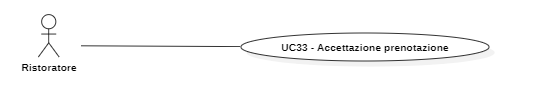
\includegraphics[scale=1]{uc33.png} \end{figure}
\begin{itemize}
\item \textbf{Attore principale:} Ristoratore.
\item \textbf{Precondizioni:}
\begin{itemize}
        \item Il ristoratore è connesso al sistema e sta visualizzando il dettaglio di una singola prenotazione (si veda UC36-Visualizzazione singola prenotazione);
        \item La prenotazione è nello stato "In attesa".
\end{itemize}
\item \textbf{Postcondizioni:} Lo stato della prenotazione diventa "Accettata".
\item \textbf{Scenario principale:}
\begin{enumerate}
    \item Il ristoratore seleziona l'opzione di accettazione della prenotazione;
    \item Il sistema aggiorna lo stato della prenotazione.
\end{enumerate}
\end{itemize}

\pagebreak
\subsubsection{UC34-Rifiuta prenotazione}
\begin{figure}[h] 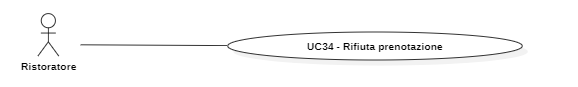
\includegraphics[scale=1]{uc34.png} \end{figure}
\begin{itemize}
\item \textbf{Attore principale:} Ristoratore.
\item \textbf{Precondizioni:}
\begin{itemize}
        \item Il ristoratore è connesso al sistema e sta visualizzando il dettaglio di una singola prenotazione (si veda UC36-Visualizzazione singola prenotazione);
        \item La prenotazione è nello stato "In attesa".
\end{itemize}
\item \textbf{Postcondizioni:} Lo stato della prenotazione diventa "Rifiutata".
\item \textbf{Scenario principale:}
\begin{enumerate}
    \item Il ristoratore seleziona l'opzione di rifiuto della prenotazione;
    \item Il ristoratore inserisce opzionalmente le motivazioni del rifiuto della prenotazione;
    \item Il sistema aggiorna lo stato della prenotazione.
\end{enumerate}
\end{itemize}

\subsubsection{UC35-Visualizzazione lista prenotazioni} % uc35 e 35.1 sono due funzionalità differenti
\begin{figure}[h] 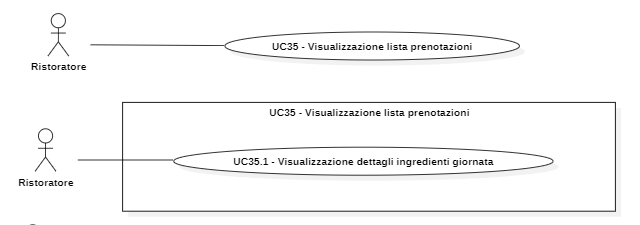
\includegraphics[scale=1]{uc35.png} \end{figure}
\begin{itemize}
\item \textbf{Attore principale:} Ristoratore.
\item \textbf{Precondizioni:} Il ristoratore è connesso al sistema.
\item \textbf{Postcondizioni:} Il ristoratore visualizza la lista delle prenotazioni (in qualsiasi stato esse si trovino) suddivise per giorno.
\item \textbf{Scenario principale:}
\begin{enumerate}
    \item Il sistema mostra le prenotazioni raggruppate per giorno.
    \item Per ogni giorno il ristoratore può consultare:
    \begin{itemize}
        \item La lista delle prenotazioni di quel particolare giorno;
        \item La lista degli ingredienti necessari per tale giorno (si veda UC35.1).
    \end{itemize}
    \item Il sistema mostra la lista delle prenotazioni inerente ad un giorno nei seguenti modi:
    \begin{itemize}
        \item Di default, vengono mostrate come prime le prenotazioni nello stato "Accettata";
        \item Il ristoratore può inoltre applicare un filtro in base allo stato della prenotazione.
    \end{itemize}
\end{enumerate}
\end{itemize}

\textbf{UC35.1-Visualizzazione dettagli ingredienti giornata} % andare quindi a creare un caso d'uso solo per il dettaglio ingredienti giornata?
\begin{itemize}
\item \textbf{Attore principale:} Ristoratore.
\item \textbf{Precondizioni:} Il ristoratore si trova nella sezione "Visualizzazione lista prenotazioni" (si veda UC35).
\item \textbf{Postcondizioni:} Il ristoratore visualizza la lista degli ingredienti.
\item \textbf{Scenario principale:}
\begin{enumerate}
    \item Il sistema mostra la vista degli ingredienti relativi alla giornata, relativamente alle prenotazioni nello stato "Accettata";
    \item Il ristoratore visualizza la lista degli ingredienti.
\end{enumerate}
\end{itemize}

\subsubsection{UC36-Visualizzazione singola prenotazione}
\begin{figure}[h] 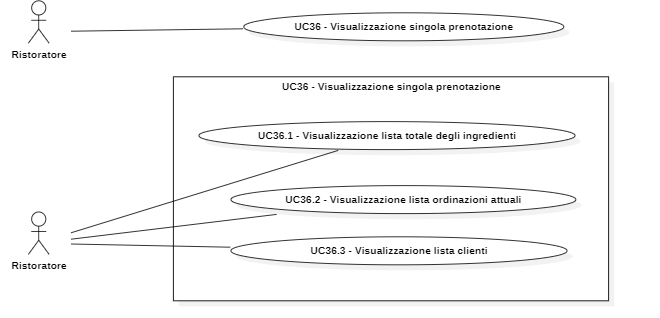
\includegraphics[scale=1]{uc36.png} \end{figure}
\begin{itemize}
    \item \textbf{Attore principale:} Ristoratore.
    \item \textbf{Precondizioni:} Il ristoratore si trova nella sezione "Visualizzazione lista prenotazioni" (si veda UC35);
    \item \textbf{Postcondizioni:} Il ristoratore visualizza le informazioni dettagliate della singola prenotazione.
    \item \textbf{Scenario principale:}
    \begin{enumerate}
        \item Il ristoratore seleziona una prenotazione da visualizzare in dettaglio.
        \item Il sistema mostra i dettagli e le informazioni relative alla prenotazione selezionata dal ristoratore:
        \begin{itemize}
            \item Username del profilo che ha effettuato la prenotazione;
            \item Giorno e orario della prenotazione;
            \item Numero di persone;
            \item Stato della prenotazione;
            \item Lista totale degli ingredienti per la ordinazione (si veda UC36.1);
            \item Lista delle ordinazioni attuali, sia confermate che non (si veda UC36.2);
            \item Lista dei clienti facenti parte della prenotazione (si veda UC36.3).
        \end{itemize}
    \end{enumerate}
\end{itemize}

\textbf{UC36.1-Visualizzazione lista totale degli ingredienti}
\begin{itemize}
    \item \textbf{Attore principale:} Ristoratore.
    \item \textbf{Precondizioni:}
    \begin{itemize}
        \item Il ristoratore si trova nella sezione "Visualizzazione singola prenotazione" (si veda UC36);
        \item Il ristoratore seleziona "Lista ingredienti per questa prenotazione".
    \end{itemize}
    \item \textbf{Postcondizioni:} Il ristoratore visualizza la lista degli ingredienti per la singola prenotazione.
    \item \textbf{Scenario principale:}
    \begin{enumerate}
        \item Il ristoratore visualizza la lista degli ingredienti che servono per completare quella prenotazione, ogni ingrediente ha una sua quantità espressa in grammi.
    \end{enumerate}
\end{itemize}

\textbf{UC36.2-Visualizzazione lista ordinazioni attuali}
\begin{itemize}
    \item \textbf{Attore principale:} Ristoratore.
    \item \textbf{Precondizioni:} Il ristoratore si trova nella sezione "Visualizzazione singola prenotazione" (si veda UC36).
    \item \textbf{Postcondizioni:} Il ristoratore visualizza la lista delle ordinazioni per la singola prenotazione.
    \item \textbf{Scenario principale:}
    \begin{enumerate}
        \item Il ristoratore seleziona l'opzione "Ordinazioni per questa prenotazione";
        \item Il ristoratore visualizza la lista delle ordinazioni che sono state effettuate dai clienti collegati a questa prenotazione nei seguenti modi:
        \begin{itemize}
            \item Di default, vengono mostrate come prime le ordinazioni nello stato "Confermata";
            \item Il ristoratore può inoltre applicare un filtro in base allo stato dell'ordinazione.
        \end{itemize}
    \end{enumerate}
\end{itemize}

\pagebreak

\textbf{UC36.3-Visualizzazione lista Clienti}
\begin{itemize}
    \item \textbf{Attore principale:} Ristoratore.
    \item \textbf{Precondizioni:}
    \begin{itemize}
        \item Il ristoratore si trova nella sezione "Visualizzazione singola prenotazione" (si veda UC36);
        \item Il ristoratore seleziona "Lista clienti".
    \end{itemize}
    \item \textbf{Postcondizioni:} Il ristoratore visualizza la lista dei clienti collegati alla singola prenotazione.
    \item \textbf{Scenario principale:}
    \begin{enumerate}
        \item Il ristoratore visualizza la lista dei clienti collegati a questa prenotazione nei seguenti modi:
        \begin{itemize}
            \item Di default, vengono mostrati per primi i clienti le cui ordinazioni sono nello stato "Confermata";
            \item Il ristoratore può inoltre applicare un filtro in base allo stato dell'ordinazione del cliente.
        \end{itemize}
    \end{enumerate}
\end{itemize}

\subsubsection{UC37-Modifica menù}
\begin{figure}[h] 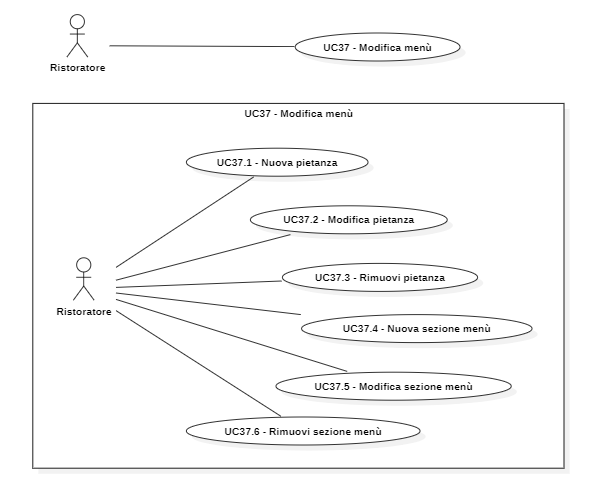
\includegraphics[scale=1]{uc37.png} \end{figure}
\begin{itemize}
    \item \textbf{Attore principale:} Ristoratore.
    \item \textbf{Precondizioni:} Il ristoratore ha effettuato l'accesso al sistema.
    \item \textbf{Postcondizioni:} Le modifiche apportate al menù sono salvate.
    \item \textbf{Scenario principale:}
    \begin{enumerate}
        \item Il ristoratore visualizza le pietanze contenute nel menù del ristorante;
        \item Il ristoratore può eseguire le seguenti operazioni di modifica:
        \begin{itemize}
           \item Aggiungere una nuova pietanza al menù (si veda UC37.1);
           \item Modificare una pietanza preesistente (si veda UC37.2);
           \item Rimuovere una pietanza dal menù (si veda UC37.3);
           \item Aggiungere una nuova sezione al menù (si veda UC37.4);
           \item Modificare una sezione del menù (si veda UC37.5);
           \item Rimuovere una sezione dal menù (si veda UC37.6);
        \end{itemize}
        \item Il ristoratore dopo aver apportato modifiche al menù le conferma;
        \item Il sistema aggiorna le informazioni sul menù del ristorante;
    \end{enumerate}
\end{itemize}

\textbf{UC37.1-Nuova pietanza}
\begin{itemize}
    \item \textbf{Attore principale:} Ristoratore.
    \item \textbf{Precondizioni:} Il ristoratore si trova nella sezione di modifica del menù (si veda UC37).
    \item \textbf{Postcondizioni:} Il ristoratore ha inserito una nuova pietanza al menù.
    \item \textbf{Scenario principale:}
    \begin{enumerate}
        \item Il ristoratore seleziona l'opzione di creazione di una nuova pietanza;
        \item Il ristoratore inserisce le informazioni relative alla pietanza:
        \begin{itemize}
            \item Il nome della pietanza;
            \item Seleziona gli ingredienti che compongono la pietanza dalla lista degli ingredienti, con la loro quantità espressa in grammi (si veda UC38 per la creazione di tale lista);
            \item Seleziona la sezione del menù a cui questo piatto appartiene.
        \end{itemize}
        \item Il ristoratore conferma l'aggiunta di una nuova pietanza al menù;
        \item Il sistema aggiorna il menù con la nuova pietanza;
        \item Il ristoratore viene reindirizzato alla schermata di modifica menù (si veda UC37).
    \end{enumerate}
\end{itemize}

\textbf{UC37.2-Modifica pietanza}
\begin{itemize}
    \item \textbf{Attore principale:} Ristoratore.
    \item \textbf{Precondizioni:} Il ristoratore si trova nella sezione di modifica del menù (si veda UC37).
    \item \textbf{Postcondizioni:} Il ristoratore ha modificato una pietanza al menù.
    \item \textbf{Scenario principale:}
    \begin{enumerate}
        \item Il ristoratore seleziona l'opzione di modifica di una pietanza;
        \item Il ristoratore modifica le informazioni relative alla pietanza:
        \begin{itemize}
            \item Il nome della pietanza;
            \item Seleziona gli ingredienti che compongono la pietanza dalla lista degli ingredienti, con la loro quantità espressa in grammi (si veda UC38 per la creazione di tale lista);
            \item Seleziona la sezione del menù a cui questo piatto appartiene.
        \end{itemize}
        \item Il ristoratore conferma le modifiche della pietanza;
        \item Il sistema aggiorna il menù con le modifiche apportate alla pietanza;
        \item Il ristoratore viene reindirizzato alla schermata di modifica menù (si veda UC37).
    \end{enumerate}
\end{itemize}

\textbf{UC37.3-Rimuovi pietanza}
\begin{itemize}
    \item \textbf{Attore principale:} Ristoratore.
    \item \textbf{Precondizioni:} Il ristoratore si trova nella sezione di modifica del menù (si veda UC37).
    \item \textbf{Postcondizioni:} La pietanza non è più presente nel menù.
    \item \textbf{Scenario principale:}
    \begin{enumerate}
        \item Il ristoratore seleziona l'opzione di eliminazione di una pietanza;
        \item Il sistema aggiorna il menù con l'eliminazione della pietanza.
        \item Il ristoratore viene reindirizzato alla schermata di modifica menù (si veda UC37).
    \end{enumerate}
\end{itemize}


\textbf{UC37.4-Nuova sezione menù}
\begin{itemize}
    \item \textbf{Attore principale:} Ristoratore.
    \item \textbf{Precondizioni:} Il ristoratore si trova nella sezione di modifica del menù (si veda UC37).
    \item \textbf{Postcondizioni:} Il ristoratore ha inserito una nuova sezione al menù.
    \item \textbf{Scenario principale:}
    \begin{enumerate}
        \item Il ristoratore seleziona l'opzione di creazione di una sezione;
        \item Il ristoratore inserisce il nome della nuova sezione;
        \item Il ristoratore conferma l'aggiunta di una nuova sezione al menù;
        \item Il sistema aggiorna il menù con la nuova seziona inserita.
    \end{enumerate}
\end{itemize}

\textbf{UC37.5-Modifica sezione menù}
\begin{itemize}
    \item \textbf{Attore principale:} Ristoratore.
    \item \textbf{Precondizioni:} Il ristoratore si trova nella sezione di modifica del menù (si veda UC37).
    \item \textbf{Postcondizioni:} Il ristoratore ha modificato una sezione al menù.
    \item \textbf{Scenario principale:}
    \begin{enumerate}
        \item Il ristoratore seleziona l'opzione di modifica di una sezione;
        \item Il ristoratore modifica il nome della sezione;
        \item Il ristoratore conferma le modifiche apportate alla sezione;
        \item Il sistema aggiorna il menù con la sezione modificata dal ristoratore.
    \end{enumerate}
\end{itemize}


\textbf{UC37.6-Rimuovi sezione menù}
\begin{itemize}
    \item \textbf{Attore principale:} Ristoratore.
    \item \textbf{Precondizioni:} Il ristoratore si trova nella sezione di modifica del menù (si veda UC37).
    \item \textbf{Postcondizioni:} La sezione non è più presente nel menù.
    \item \textbf{Scenario principale:}
    \begin{enumerate}
        \item Il ristoratore seleziona l'opzione di eliminazione di una sezione;
        \item Il sistema aggiorna il menù con l'eliminazione della sezione.
    \end{enumerate}
\end{itemize}

\subsubsection{UC38-Modifica lista degli ingredienti}
\begin{figure}[h] 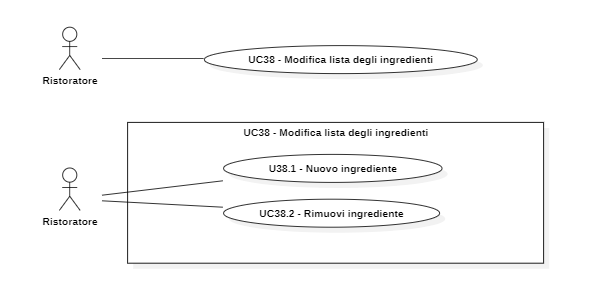
\includegraphics[scale=1]{uc38.png} \end{figure}
\begin{itemize}
    \item \textbf{Attore principale:} Ristoratore.
    \item \textbf{Precondizioni:} Il ristoratore ha effettuato l'accesso al sistema.
    \item \textbf{Postcondizioni:} Le modifiche apportate sono state salvate.
    \item \textbf{Scenario principale:}
    \begin{enumerate}
        \item Il ristoratore visualizza la lista degli ingredienti del ristorante;
        \item Il ristoratore può eseguire le seguenti operazioni:
        \begin{itemize}
           \item Aggiungere un nuovo ingrediente alla lista (si veda UC38.1);
           \item Rimuovere un ingrediente presente nella lista (si veda UC38.2).
        \end{itemize}
    \item Il ristoratore conferma le modifiche apportate alla lista degli ingredienti;
    \item Il sistema aggiorna la lista degli ingredienti;
    \item Il ristoratore viene reindirizzato alla dashboard.
    \end{enumerate}
\end{itemize}

\pagebreak
\textbf{UC38.1-Nuovo ingrediente}
\begin{itemize}
    \item \textbf{Attore principale:} Ristoratore.
    \item \textbf{Precondizioni:} Il ristoratore si trova nella sezione di modifica della lista ingredienti (si veda UC38).
    \item \textbf{Postcondizioni:} Viene inserito un nuovo ingrediente nella lista degli ingredienti.
    \item \textbf{Scenario principale:}
    \begin{enumerate}
        \item Il ristoratore seleziona l'opzione di creazione di un nuovo ingrediente;
        \item Il ristoratore compila il seguente form contenente le informazioni relative alla pietanza:
        \begin{itemize}
            \item Il nome dell'ingrediente;
            \item Opzionalmente seleziona gli allergeni contenuti all'interno di quell'ingrediente da una lista fornita dal sistema.
        \end{itemize}
        \item Il ristoratore conferma la creazione di un nuovo ingrediente;
        \item Il sistema aggiorna la lista degli ingredienti con il nuovo ingrediente;
        \item Il ristoratore viene reindirizzato alla schermata di modifica della lista ingredienti (si veda UC38).
    \end{enumerate}
\end{itemize}


\textbf{UC38.2-Rimuovi ingrediente}
\begin{itemize}
    \item \textbf{Attore principale:} Ristoratore.
    \item \textbf{Precondizioni:} Il ristoratore si trova nella sezione di gestione della lista ingredienti (si veda UC38).
    \item \textbf{Postcondizioni:} L'ingrediente viene rimosso dalla lista degli ingredienti.
    \item \textbf{Scenario principale:}
    \begin{enumerate}
        \item Il ristoratore seleziona l'opzione di eliminazione un ingrediente;
        \item Il sistema aggiorna la lista con l'eliminazione dell'ingrediente;
        \item Il ristoratore viene reindirizzato alla schermata di modifica della lista ingredienti (si veda UC38).
    \end{enumerate}
\end{itemize}
\pagebreak
\subsubsection{UC39-Visualizzazione recensioni ristorante} % analizzare più in dettaglio (grazie al *****)
\begin{figure}[h] 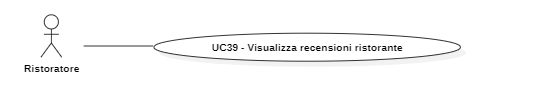
\includegraphics[scale=1]{uc39.png} \end{figure}
\begin{itemize}
\item \textbf{Attore principale:} Ristoratore.
\item \textbf{Precondizioni:} Il ristoratore è connesso al sistema.
\item \textbf{Postcondizioni:} Il ristoratore visualizza le ultime 5 recensioni fatte in ordine temporale decrescente dai clienti.
\item \textbf{Scenario principale:}
\begin{enumerate}
    \item Il ristoratore seleziona la funzionalità di visualizzazione delle recensioni fatte dai clienti sulla loro esperienza presso il ristorante;
    \item Di default, se presenti più di 5 recensioni, il sistema ne presenta una lista con le ultime 5 fatte in ordine temporale decrescente;
    \item Il ristoratore visualizza le suddette recensioni, corredate dalle seguenti informazioni:
    \begin{itemize}
        \item Un voto da 1 a 5 sul menù;
        \item Un voto da 1 a 5 sul servizio;
        \item Un voto da 1 a 5 sul prezzo;
        \item Un eventuale commento testuale.
    \end{itemize}
\end{enumerate}
\end{itemize}

\subsubsection{UC40-Gestione pagamento conto}
\begin{figure}[h] 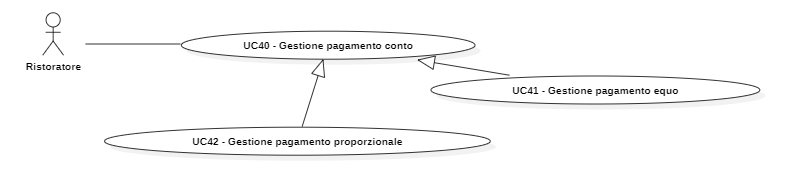
\includegraphics[scale=.7]{uc40.png} \end{figure}
\begin{itemize}
    \item \textbf{Attore principale:} Ristoratore.
    \item \textbf{Precondizioni:}
    \begin{itemize}
        \item Il ristoratore è connesso al sistema e si trova nella sezione di visualizzazione di una singola prenotazione (si veda UC36);
        \item Un cliente ha selezionato la modalità di divisione del conto (si veda UC27).
    \end{itemize}
    \item \textbf{Postcondizioni:} Rispettando la modalità di divisione del conto, una parte o il totale del conto della prenotazione è segnato come pagato.
    \item \textbf{Scenario principale:}
    \begin{enumerate}
        \item Il sistema mostra gli ordini o le persone nello stato "Pagato" e "Non pagato", elencando per prime quelle nello stato "Non pagato";
        \item Il ristoratore può selezionare un ordine o una persona e segnarla come pagata;
        \item Il sistema aggiorna lo stato dell'ordine o della persona a "Pagato";
        \item Quando tutte le ordinazioni o persone hanno pagato allora la prenotazione va nello stato "Pagata".
    \end{enumerate}
    \item \textbf{Specializzazioni:}
        \begin{itemize}
            \item UC41-Pagamento equo;
            \item UC42-Pagamento proporzionale.
        \end{itemize}
\end{itemize}

\subsubsection{UC41-Gestione pagamento equo}
\begin{itemize}
    \item \textbf{Descrizione:} Pagamento equo del totale di tutti gli ordini, ovvero "alla romana".
    \item \textbf{Attore principale:} Ristoratore.
    \item \textbf{Precondizioni:}
    \begin{itemize}
        \item Il ristoratore è connesso al sistema e si trova nella sezione di visualizzazione di una singola prenotazione (si veda UC36);
        \item Un cliente ha selezionato la modalità di divisione del conto equa (si veda UC27).
    \end{itemize}
    \item \textbf{Postcondizioni:} Il o i profili selezionati sono segnati come pagati.
    \item \textbf{Scenario principale:}
    \begin{enumerate}
        \item Il sistema mostra le persone nello stato "Pagato" e "Non pagato", elencando per prime quelle nello stato "Non pagato";
        \item Il ristoratore può selezionare una persona o più persone e segnarle come pagate;
        \item Il sistema aggiorna lo stato delle persone a "Pagato";
        \item Quando tutte le persone hanno pagato allora la prenotazione va nello stato "Pagata".
    \end{enumerate}
\end{itemize}

\subsubsection{UC42-Gestione pagamento proporzionale}
\begin{itemize}
    \item \textbf{Descrizione:} Pagamento proporzionale delle ordinazioni, ovvero i clienti selezionano gli ordini che vogliono pagare (anche di altri clienti).
    \item \textbf{Attore principale:} Ristoratore.
    \begin{itemize}
        \item Il ristoratore è connesso al sistema e si trova nella sezione di visualizzazione di una singola prenotazione (si veda UC36);
        \item Un cliente ha selezionato la modalità di divisione del conto proporzionale (si veda UC27).
    \end{itemize}
    \item \textbf{Postcondizioni:} Una o più ordinazioni selezionate sono segnate come pagate.
    \item \textbf{Scenario principale:}
    \begin{enumerate}
        \item Il sistema mostra le ordinazioni nello stato "Pagato" e "Non pagato", elencando per prime quelle nello stato "Non pagato";
        \item Il ristoratore può selezionare una o più ordinazioni e segnarle come pagate;
        \item Il sistema aggiorna lo stato delle ordinazioni a "Pagato";
        \item Quando tutte le ordinazioni sono segnate come pagate allora la prenotazione va nello stato "Pagato".
    \end{enumerate}
\end{itemize}

\subsubsection{UC43-Visualizzazione notifica cliente ha confermato l'ordinazione}
\begin{figure}[h] 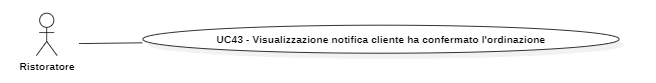
\includegraphics[scale=1]{uc43.png} \end{figure}
\begin{itemize}
\item \textbf{Attore principale:} Ristoratore.
\item \textbf{Precondizioni:} Il cliente ha confermato l'ordinazione (si veda UC23.3).
\item \textbf{Postcondizioni:} Il ristoratore visualizza una notifica relativa alla conferma dell'ordinazione.
\item \textbf{Scenario principale:}
\begin{enumerate}
    \item Il sistema vede che è stata confermata un'ordinazione dal cliente;
    \item Il sistema invia al ristoratore una notifica relativa alla conferma dell'ordinazione;
    \item Il ristoratore visualizza la notifica relativa all'ordinazione.
\end{enumerate}
\end{itemize}

\subsubsection{UC44-Visualizzazione notifica cliente ha annullato la prenotazione}
\begin{figure}[h] 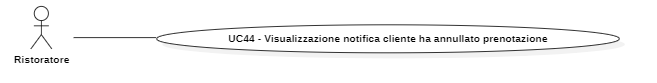
\includegraphics[scale=1]{uc44.png} \end{figure}
\begin{itemize}
\item \textbf{Attore principale:} Ristoratore.
\item \textbf{Precondizioni:} Il cliente ha annullato la prenotazione (si veda UC21).
\item \textbf{Postcondizioni:} Il ristoratore visualizza una notifica relativa all'annullamento della prenotazione.
\item \textbf{Scenario principale:}
\begin{enumerate}
    \item Il sistema vede che è stata annullata una prenotazione dal cliente;
    \item Il sistema invia al ristoratore una notifica relativa all'annullamento della prenotazione;
    \item Il ristoratore visualizza la notifica relativa all'annullamento della prenotazione.
\end{enumerate}
\end{itemize}

\pagebreak
\subsubsection{UC45-Visualizzazione notifica nuova prenotazione in arrivo}
\begin{figure}[h] 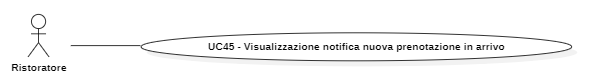
\includegraphics[scale=1]{uc45.png} \end{figure}
\begin{itemize}
\item \textbf{Attore principale:} Ristoratore.
\item \textbf{Precondizioni:} Il cliente ha effettuato una prenotazione (si veda UC19).
\item \textbf{Postcondizioni:} Il ristoratore visualizza una notifica relativa alla prenotazione di un tavolo.
\item \textbf{Scenario principale:}
\begin{enumerate}
    \item Il sistema vede che è stata effettuata una prenotazione dal cliente;
    \item Il sistema invia al ristoratore una notifica relativa ad una nuova prenotazione;
    \item Il ristoratore visualizza la notifica relativa alla nuova prenotazione.
\end{enumerate}
\end{itemize}

\subsubsection{UC46-Visualizzazione notifica nuova recensione}
\begin{figure}[h] 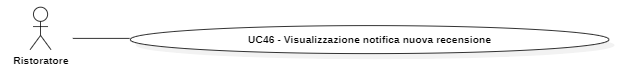
\includegraphics[scale=1]{uc46.png} \end{figure}
\begin{itemize}
\item \textbf{Attore principale:} Ristoratore.
\item \textbf{Precondizioni:} Il cliente ha lasciato una recensione (si veda UC29).
\item \textbf{Postcondizioni:} Il ristoratore visualizza una notifica relativa alla recensione.
\item \textbf{Scenario principale:}
\begin{enumerate}
    \item Il sistema vede che è stata lasciata una recensione dal cliente;
    \item Il sistema invia al ristoratore una notifica relativa alla nuova recensione;
    \item Il ristoratore visualizza la notifica relativa alla nuova recensione.
\end{enumerate}
\end{itemize}

\pagebreak
\subsubsection{UC47-Visualizzazione notifica cliente ha pagato in app}
\begin{figure}[h] 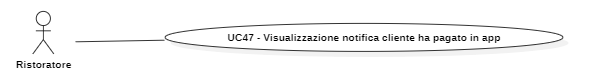
\includegraphics[scale=1]{uc47.png} \end{figure}
\begin{itemize}
\item \textbf{Attore principale:} Ristoratore.
\item \textbf{Precondizioni:} Il cliente ha effettuato un pagamento in app (si veda UC28).
\item \textbf{Postcondizioni:} Il ristoratore visualizza una notifica relativa al pagamento in app.
\item \textbf{Scenario principale:}
\begin{enumerate}
    \item Il sistema vede che è stata pagata un'ordinazione dal cliente;
    \item Il sistema invia al ristoratore una notifica relativa ad un pagamento;
    \item Il ristoratore visualizza la notifica relativa al pagamento.
\end{enumerate}
\end{itemize}

\subsubsection{UC48-Visualizzazione notifica ricezione messaggio in chat}
\begin{figure}[h] 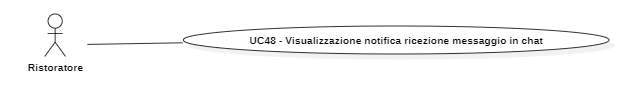
\includegraphics[scale=1]{uc48.png} \end{figure}
\begin{itemize}
\item \textbf{Attore principale:} Ristoratore.
\item \textbf{Precondizioni:}
\begin{itemize}
    \item Il cliente ha avviato la chat con il ristoratore (si veda UC49);
    \item Il cliente ha inviato un messaggio al ristoratore (si veda UC50.1).
\end{itemize}
\item \textbf{Postcondizioni:} Il ristoratore visualizza una notifica relativa alla ricezione di un messaggio in chat.
\item \textbf{Scenario principale:}
\begin{enumerate}
    \item Il sistema vede che è stato inviato un messaggio dal cliente;
    \item Il sistema invia al ristoratore una notifica relativa al messaggio;
    \item Il ristoratore visualizza la notifica relativa al messaggio.
\end{enumerate}
\end{itemize}



% chat

\textbf{UC49-Avvia chat}
\begin{itemize}
\item \textbf{Attore principale:} Cliente.
\item \textbf{Precondizioni:} È in corso una prenotazione e il cliente non ha ancora avviato la chat. % TODO non so come mettere a parole che deve essere il cliente a voler comunicare con il ristoratore
\item \textbf{Postcondizioni:} Diventa possibile comunicare con il ristoratore.
\item \textbf{Scenario secondario:}
\begin{enumerate}
    \item Il cliente ha dei dubbi che vuole chiarire.
    \item Il cliente preme il tasto di avvio della chat.
    \item Il sistema crea la chat.
    \item Diventa possibile comunicare bidirezionalmente tra il/i cliente/clienti e il ristoratore. 
\end{enumerate}
\end{itemize}

\textbf{UC50-Apertura chat}
\begin{itemize}
\item \textbf{Attore principale:} Cliente / Ristoratore
\item \textbf{Precondizioni:}
\item \textbf{Postcondizioni:}
\item \textbf{Scenario secondario:}
\begin{enumerate}
    \item
\end{enumerate}
\end{itemize}

\textbf{UC50.1-Invio messaggio}
\begin{itemize}
\item \textbf{Attore principale:} Cliente / Ristoratore
\item \textbf{Precondizioni:}
\item \textbf{Postcondizioni:}
\item \textbf{Scenario secondario:}
\begin{enumerate}
    \item
\end{enumerate}
\end{itemize}

\textbf{UC50.2-Lettura messaggio}
\begin{itemize}
\item \textbf{Attore principale:} Cliente / Ristoratore
\item \textbf{Precondizioni:}
\item \textbf{Postcondizioni:}
\item \textbf{Scenario secondario:}
\begin{enumerate}
    \item
\end{enumerate}
\end{itemize}

